% NOTE - this is only a template without real arguments
\begin{entry}{Callback Class Troubleshooting/Repair}{Aug 23, 2021}
    \objective 
    
    TS\&R Callback classes

    \outline

    \begin{itemize}
        \item Contact PNNL
        \item Fix EdmMeasurementProcessor
        \item Fix EdmTimeKeeper
        \item Fix EdmOnClose

    \end{itemize}

    \procedures
    
    Currently using the old callback functions to call the \verb"on_message" method of each callback class. Frankly, this works
    perfectly well and is invisible to the user and developers in most cases. It does require function definitions and
    global variables and weird stuff that I'd prefer to remove. So, after contacting PNNL, figure out the issue and fix
    the classes.

    \parameters
    
    N/A

    \observations
    
    The issue was in the way I was gathering the simulation ID. I reused code that I'd never actually USED in the old
    script, and this code turns out not to have been working this whole time. Turns out there's an easier way to do it
    anyways; I just have to start the simulation first, and then get the ID, then use that to instantiate everything. It
    works fine.

    The EdmMeasurementProcessor works fine. The EdmTimekeeper also works fine, but differently from the old callback
    function: it uses a subscription to the log topic and therefore I have to filter out the messages that include
    timestep incrementation manually. This is done, and works more or less fine. The EdmOnClose isn't yet working since
    there's no obvious subscription topic for it. I may have to settle for the callback function on this one, but
    I'm contacting PNNL to be sure.

    May be a timekeeping bug. The timestep increments before the measurement processor; but, the measurement processor
    uses its own timestamp anyways. Timecodes seem to be 2 off. Will need to do some rigorous testing at the end of
    Phase 1 to fully verify what's going on and make sure that inputs are being reflected in the outputs at the proper
    time (which should be the timestep after they're injected.)

    \data
    
    N/A

    \results
    
    EdmMeasurementProcessor and EdmTimeKeeper working as intended. EdmTimeKeeper filtering function needs cleaned up.
    EdmOnClose not yet implemented. Awaiting PNNL support.

\end{entry}


%\begin{entry}{CMake Error running EGOT-DCM Dockerfile}{Dec 02, 2020}
%    \objective
%
%    Determine the cause of the CMake error while running the dockerfile and modify file to get it to successfully build.
%
%    \outline
%
%    \begin{itemize}
%        \item Try running to see if it was just Lorry or a machine issue.
%        \item If it is a machine issue, modify configurations to ensure interoperability.
%        \item If I get the error track down its cause and modify dockerfile to fix.
%        \item Repeat until all builds are successful.
%    \end{itemize}
%
%    \procedures
%
%    \begin{itemize}
%        \item \mint{console}|git clone https://github.com/EGoT-DCS-SunSpec-Modbus|
%        \item \mint{console}|docker build -f Dockerfile.buster -t egot-dcs .|
%        \item \mint{console}|docker container run -i egot-dcs|
%    \end{itemize}
%
%    \observations
%
%    \begin{error}{Cmake Error: No CMAKE\_CXX\_COMPILER found}
%        \begin{figure}[H]
%            \centering
%            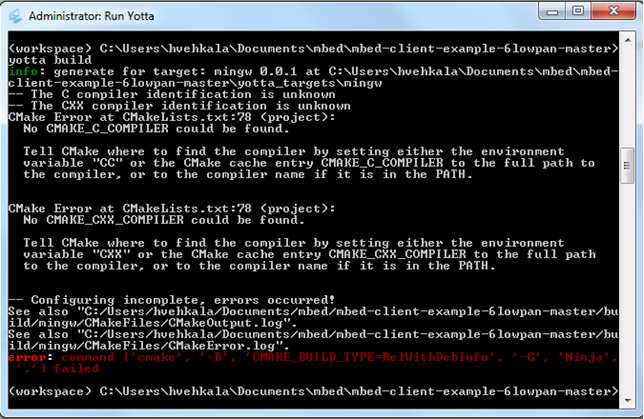
\includegraphics[height=4in]{Fall2020/Figures/cmake_error.png}
%        \end{figure}
%
%        Solution: what you need to do found at \cite{CMAKE-Forum}
%    \end{error}
%
%    \results
%
%    Short: No.
%
%    Long: Well...
%
%
%\end{entry}